\documentclass[12pt]{article}
\pdfoutput=1

\usepackage{draft} 
\usepackage{hyperref}
\usepackage{graphicx,color,subfig}
\usepackage{cite}
\usepackage{mciteplus}
\usepackage{skak}
\usepackage{empheq}
\usepackage{anyfontsize}
% Use Chancery Font
\DeclareFontFamily{OT1}{pzc}{}
\DeclareFontShape{OT1}{pzc}{m}{it}{<-> s * [1.10] pzcmi7t}{}
\DeclareMathAlphabet{\mathpzc}{OT1}{pzc}{m}{it}

%\usepackage{chngcntr}
%\counterwithout{equation}{section}

\newcommand{\wt}[1]{\widetilde{#1}}
\newcommand{\vv}[1]{\left\langle #1 \right\rangle}
\newcommand{\un}[1]{\underline{#1}}
\newcommand{\BL}[1]{{ {\color{blue}[#1]}}}
\newcommand{\im}{\mathrm{Im}}


\newcommand{\fixme}[1]{{\bf {\color{red}[#1]}}}
\def\be#1\ee{\begin{align}#1\end{align}}
\newcommand\nn{\nonumber}

\begin{document}

 
\unitlength = .8mm




\section{The strategy}

We aim to evaluate a string amplitude (free energy) of the form
\ie
{\cal F} = \int_{\cal M} d\mu,
\fe 
where ${\cal M}$ is a suitable moduli space (say of the genus $g$ Riemann surface) and $d\mu$ is a positive measure. The idea is to compare it with
\ie
{\cal F}_0 = \int_{\cal M} d\mu_0
\fe
of a solvable model, and express
\ie
{\cal F} = {\cal F}_0 \left\langle {d\mu\over d\mu_0} \right\rangle_0,
\fe
where 
\ie
\left\langle f \right\rangle_0 = { \int_{\cal M} d\mu_0 \, f\over  \int_{\cal M} d\mu_0}
\fe
can be numerically evaluated by Monte Carlo sampling of $f$ over ${\cal M}$ with probability measure $d\mu_0$.


\section{The moduli space}

The moduli space ${\cal M}_g$ of genus $g$ Riemann surface can be viewed as the base of the obvious fibration
\ie
\pi: {\cal M}_{g,1} \to {\cal M}_g,
\fe
and ${\cal M}_{g,1}$ can be parameterized via the moduli space ${\cal M}_{g,1}^{\rm comb}$ of metric ribbon graphs, via Kontsevich's isomorphism
\ie
{\cal M}_{g,1}\times \mathbb{R}_+ \xrightarrow{\sim} {\cal M}_{g,1}^{\rm comb}.
\fe
The explicit ribbon graph is constructed by finding the Strebel differential $\omega = \varphi(z) dz^2$, whose zeros of degree $d$ corresponding to vertices of the graph with valence $d+2$. The defining property of $\omega$ is such that all of its horizontal trajectories, along which $\varphi(z(s)) ({dz\over ds})^2\in \mathbb{R}_+$, are closed or end on a zero. The length of a closed horizontal trajectory $\C$ is equal to 
\ie
\ell(\C) = \oint_\gamma \sqrt{\varphi(z)}\, dz,
\fe
and is constant along a continuous family of closed horizontal trajectories. In the case of one puncture, all closed horizontal trajectories are homologous and enclose the puncture where $\varphi(z)$ has a double pole.

At a generic point in the moduli space, the ribbon graph in question has only cubic vertices, and Euler characteristic $V-E+F = 2-2g$ with $3V=2E$ and $F=1$. So the number of vertices is $V=4g-2$, and the number of edges is $E=6g-3$. %There are $3g-3$ linearly independent holomorphic quadratic differentials.

Consider the example of a 1-punctured torus, parameterized by the holomorphic coordinate $z\sim z + 2\pi \sim z + 2\pi \tau$ with the puncture at $z=0$. The Strebel differential is of the form
\ie
\omega = \ell^2 \left( {\cal P}_\tau(z) - a \right) dz^2,
\fe
where ${\cal P}_\tau(z)$ is the Weierstrass elliptic function which has a double zero at $z=0$,
\ie
{\cal P}_\tau(z) = {1\over z^2} + \sum_{(m,n)\not=(0,0)} \left[ {1\over (z-2\pi (m + n \tau))^2} - {1\over (2\pi (m + n \tau))^2}\right].
\fe 
%$a$ is chosen to be one of $e_1, e_2, e_3$, where
%\ie
%e_1 = {\cal P}_\tau(\pi),~~~~ e_2 = {\cal P}_\tau(\pi \tau),~~~~ e_3 = {\cal P}_\tau(\pi+\pi\tau).
%\fe
The constant $a$ is determined by $\tau$ by the condition that the horizontal trajectories are closed. %This essentially amounts to demanding that $\oint_\C \sqrt{\omega}$ for $\C$ enclosing $z=0$ is real and positive.


Rather than mapping metric graph data to plumbing parameters and computing CFT correlators from conformal blocks, the strategy is to directly computing CFT observable in terms of the metric graph data. For instance, the torus partition function of a free boson $X$ can be represented, modulo Weyl anomaly, as
\ie\label{zthetas}
Z(\theta_1, \theta_2) &= \int [DX(\sigma)]_{0<\sigma<2\pi} \Psi_1[X(\sigma)] \prod_{0<\sigma<\theta_1} \delta(X(\sigma)-X(\pi+\theta_1-\sigma))
\\
&~~~\times \prod_{\theta_1<\sigma< \theta_2} \delta(X(\sigma)-X(\pi+\theta_1+\theta_2 - \sigma))  \prod_{\theta_2<\sigma< \pi} \delta(X(\sigma)-X(2\pi+\theta_2 - \sigma)).
\fe
Here $0<\theta_1<\theta_2<2\pi$ are related to the lengths $\ell_1, \ell_2, \ell_3$ of the metric graph by $\theta_1 = \pi {\ell_1\over \ell_1+\ell_2+\ell_3}$ and $\theta_2 = \pi {\ell_1+\ell_2 \over \ell_1+\ell_2+\ell_3}$. $\Psi_1[X(\sigma)]$ is the wave functional of the identity operator. As in (2.8.23) of Polchinski, 
\ie\label{psionefx}
\Psi_1[X(\sigma)] \propto \exp\left( - {1\over \A'}\sum_{m\geq 1} m X_m X_{-m} \right),
\fe
where $X_m$ is the $m$-th Fourier mode of $X(\sigma)$.

To obtain the genus 2 partition function, the ribbon graph at a generic point in the moduli space has 6 cubic vertices and 9 edges. The partition function can be obtained by integrating $\Psi_1[X(\sigma)]$ with the identification of $X$ on pairs of 18 segments of the unit circle.


\section{Application to $c=1$ string theory}

The idea is to take $d\mu_R$ to be the measure associated with the free energy of $c=1$ string theory at inverse temperature $\B = 2\pi R$, and compare the measure at different values of $R$. Explicitly, as in (4.97) of the string notes, we have on ${\cal M}_g$
\ie
d\mu_R = \prod_{k=1}^{3g-3} i d\tau^k \wedge d\bar\tau^k \left\langle \prod_{k=1}^{3g-3} {\cal B}_{\bar\tau^k} {\cal B}_{\tau^k}  \right\rangle_\Sigma,
\fe
which is a positive measure. The correlator is evaluated for the matter CFT that consists of $c=25$ Liouville theory and a compact boson of radius $R$. It follows that
\ie\label{dmuratio}
{d\mu_R\over d\mu_{R_0}} = {Z_{R}(\Sigma)\over Z_{R_0}(\Sigma)},
\fe
where $Z_R(\Sigma)$ is the partition function of the compact boson of radius $R$ on the Riemann surface $\Sigma$. Note that the Weyl anomaly cancels between the numerator and the denominator and so the RHS is well-defined.

Typically, the RHS of (\ref{dmuratio}) is not hard to compute. The main challenge is to find an algorithm for sampling ${\cal M}_g$, say with Metropolis algorithm, subject to the probability measure $d\mu_{R_0}$.

In the case of the genus 2 free energy, there is an expression in terms of the period matrix $\Omega_{IJ}$,
\ie
{\cal F}_2(R) = \int_{{\cal M}_2} \left| \Phi(\Omega) d\Omega_{11} d\Omega_{22} d\Omega_{12} \right|^2 {V_{26}\over (4\pi^2 \A')^{26} (\det{\rm Im}\Omega)^{13} Z_{26}(\Sigma) } {Z_{1,R}(\Sigma) Z_L(\Sigma)},
\fe
where $\Phi(\Omega)=2\pi i/\chi_{10}(\Omega)$ as in (4.109) of the string notes, $Z_{26}(\Sigma)$ is the genus two partition function of 26 noncompact free bosons with target space volume $V_{26}$, $Z_{1,R}(\Sigma)$ is the partition function of a compact boson at radius $R$, and $Z_L(\Sigma)$ is the $c=25$ Liouville CFT partition function. Each partition function is subject to the Weyl anomaly, which cancels in the combination $Z_{1,R}(\Sigma) Z_L(\Sigma)/Z_{26}(\Sigma)$.


\section{$\Psi_1$ of Liouville CFT}


The Euclidean action of Liouville theory is
\ie
S_L = {1\over 4\pi} \int d^2\sigma \sqrt{g} (g^{ab} \partial_a \partial_b \phi + Q R \phi + 4\pi \mu e^{2b\phi}),
\fe
where $Q=b+b^{-1}$. On the cylinder, the Hamiltonian reads
\ie
H = \int d\sigma \left[ \pi \Pi_\phi^2 + {1\over 4\pi } (\partial_\sigma\phi)^2 + :\mu e^{2b\phi}: \right],
\fe
where $: ~:$ is the normal ordering defined via the mode expansion
\ie{}
& \phi = \sum_{n\in \mathbb Z} {1\over \sqrt{2|n|} } (a_n + a_{-n}^\dagger ) e^{in\sigma} ,
\\
& \Pi_\phi = {-i\over 2\pi} \sum_{n\in \mathbb Z} \sqrt{|n|\over 2 } (a_n - a_{-n}^\dagger ) e^{in\sigma}.
\fe
The exactness of this Hamiltonian can be justified through its commutation relation with the Virasoro generators defined by the holomorphic stress-energy tensor of the form
\ie
T = - :\partial \phi \partial \phi : + Q \partial^2\phi.
\fe
We could consider alternatively the regularized Hamiltonian defined by discretizing space,
\ie
H = \sum_{i=1}^N \left[ {N\over 2} \Pi(i)^2 + {N\over 2(2\pi)^2} (\phi(i+1)-\phi(i))^2 + \mu {2\pi\over N} e^{2b\phi(i)} \right],
\fe
where $\phi(N+1)\equiv \phi(1)$, $[\phi(i), \Pi(j)] = i \delta_{ij}$, and seek the identity wave function $\Psi_1(\phi(1), \cdots, \phi(N))$. 

Note however that $\Psi_1$ is not the ground state, but rather the analytic continuation of a scattering state of real Liouville momentum $P$ to $P=i {Q\over 2}$. The energy of $\Psi_1$ on the cylinder is $H = - {1 \over 12} - {Q^2\over 2}$. Moreover, $\Psi_1$ is not normalizable and blows up exponentially in the large field region $\phi\to -\infty$ as $\Psi_1 \sim e^{-{Q\over 2} \phi}$. This leads to a divergence in the zero mode integration that is likely cancelled by the Weyl anomaly due to the Weyl frame of the metric associated with the ribbon graph/Strebel differential.


\section{The partition function of free boson CFT from $\Psi_1$}

Discretizing the unit circle into $L$ sites, we consider the approximation of (\ref{psionefx}),
\ie
\Psi_1[X] &\propto \exp\left[ - {1\over \pi \A' L} \sum_{m=1}^L \sin {\pi m \over L} \sum_{k,\ell=1}^L X(k) X(\ell) e^{2\pi i {m\over L} (k-\ell)} \right]
\\
&= \exp\left[ - {1\over \pi \A' L} \sum_{k,n=1}^L X(n) X(n+k) { \sin {\pi\over L} \over \cos{2\pi k\over L} - \cos{\pi\over L}} \right] .
\fe
We will assume that $L$ is even. Next we split $\tfrac{L}{ 2} =\ell_1 + \ell_2 + \ell_3$, where each $\ell_i$ is a positive integer, and make the identification
\ie\label{pairthree}
& X(\tfrac{L}{2} + \ell_1+1 - n) = X(n),~~~~ 1\leq n \leq \ell_1,
\\
& X(\tfrac{L}{2} + 2 \ell_1 + \ell_2 +1 - n) = X(n),~~~~ \ell_1+1 \leq n \leq \ell_1 + \ell_2,
\\
& X(L+\ell_1 + \ell_2+1 - n) = X(n),~~~~ \ell_1+\ell_2+1 \leq n \leq \tfrac{L}{2},
\fe
as a discretized version of (\ref{zthetas}). Finally, we perform the integration with respect to the remaining independent variables $X(n)$, $1\leq n \leq \tfrac{L}{2}$.

After imposing the constraint (\ref{pairthree}), we can write $\Psi_1[X]$ as proportional to
\ie
\exp\left[ - \sum_{k,\ell=1}^{L\over 2} A_{k\ell} X(k) X(\ell) \right],
\fe
where the eigenvalues of the matrix $A_{k\ell}$ are positive except for a single zero. The integration over $X(k)$, $1\leq k\leq {L\over 2}$ then produces, up to a constant normalization factor, the determinant
\ie\label{detprime}
Z_L(t_1, t_2, t_3) = ({\det}' A_{k\ell})^{-{1\over 2}},
\fe
where $t_i\equiv 2\ell_i /L$ with $t_1+t_2+t_3=1$, and the prime stands for removing the zero mode. This is explicitly evaluated in ``discretized wave functional.nb'' in two different ways that give the same answer.

In the limit $L\to \infty$, $Z_L$ is divergent. There are two sources for the divergence. One is due to the discretization scheme and the normalization of the Gaussian measure, and should go like $\exp(const\cdot L)$. The other is due to the Weyl anomaly associated with the surface defined by the Strebel differential, and is universal. In particular, namely a cubic vertex of the ribbon graph, the metric goes like $ds^2 =e^{2\omega} dz d\bar z \sim |z| dz d\bar z$, and so $\omega \sim {1\over 2} \log|z|$. Need a puncture, on the otherhand, we have $\omega \sim - \log|z|$. The Weyl anomaly factor in going from the flat metric to the ribbon graph metric on the torus is $e^{S_L}$ with the linear dilaton action $S_L$ given simply by
\ie\label{slact}
S_L = {1\over 12\pi} \int_{T^2} d^2z \,\partial\omega \bar\partial\omega.
\fe
As $\partial \omega \sim {1\over 4z}$ near a cubic vertex, and $\partial\omega\sim - {1\over 2z}$ near a puncture, we get logarithmic divergence
\ie
S_L \sim  {1\over 12\pi} \cdot {2\cdot 2\pi}  \left( 2\cdot {1\over 4^2} \log {1\over \delta} + {1\over 2^2} \log {1\over \epsilon} \right)  , %= {1\over 8} \log {1\over \delta},
\fe
where $\delta$ and $\epsilon$ are the cutoff parameters near the pair of cubic vertex points and the puncture respectively. Note that the coefficient of the log divergence is independent from the moduli.

% is a small cutoff parameter of order $\sim L^{-1}$. 
\subsection{Torus one point function: $\partial X \bar \partial X$}
\label{subsec:dXbdX}
Let's consider the torus one point function, for example of $\partial X \bar\partial X$. This is a weight $(1,1)$ primary operator, so
\ie
\langle :\partial X \bar \partial X:(0) \rangle_{T^2(t_1,t_2)} = |\widehat f(0)|^{-2} \langle  :\partial X \bar \partial X:(0) \rangle_{D^2(t_1,t_2)},
\fe
where the correlator on the RHS can be approximately computed as 
\ie
\propto \int \left[ \prod_{k=1}^L dX(k) \right] \Psi_{\partial X \bar\partial X}[X(k)] \delta_{\text{identification}},
\fe
with $\delta_{\text{identification}}$ corresponding to the rules (\ref{pairthree}). The wavefunctional corresponding to the (normal ordered) operator $\partial X \bar \partial X$ inserted at the origin of the disk is given by Polchinski (2.8.28) and the paragraph below it as
\ie
\Psi_{\partial X \bar\partial X}[X(\sigma)] \propto (X_1 X_{-1} - \frac{\A'}{2} )\exp \left(-\frac{1}{\A'} \sum_{m\geq 1} mX_m X_{-m}\right).
\fe
The gaussian factor is the same as in (\ref{psionefx}), while the prefactor can be approximated in the discretization scheme as 
\ie
X_1 X_{-1} \sim \frac{1}{L^2} \sum_{k,\ell = 1}^L X(k) X(\ell) e^{\frac{2\pi i}{L}(k-\ell)},
\fe
which we can denote after applying the identification rules as
\ie
X_1 X_{-1} \delta_{\text{identification}} \sim \sum_{k,\ell = 1}^{L/2}  C_{k\ell} X(k) X(\ell).
\fe
If we denote the shift used in the identification rule (\ref{pairthree}) as
\ie
\label{shiftRule}
s(n) = 
	\begin{cases}
	\frac{L}{2}+\ell_1+1, \qquad 1 \leq n \leq \ell_1\\
	\frac{L}{2}+\ell_2+2\ell_1+1, \qquad \ell_1+1 \leq n \leq \ell_1+\ell_2\\
	\frac{L}{2}+\ell_3+2\ell_2+2\ell_1+1, \qquad \ell_1+\ell_2+1 \leq n \leq \frac{L}{2}
	\end{cases}
\fe
then 
\ie
C_{k\ell} = \frac{1}{L^2} \left(e^{\frac{2\pi i}{L} (k-\ell)} + e^{-\frac{2\pi i}{L}(k-\ell-s(k)+s(\ell))} +e^{\frac{2\pi i}{L}(k+\ell - s(\ell)) }+e^{-\frac{2\pi i}{L}(k+\ell - s(k)) }\right).
\fe
Finally, we wish to evaluate 
\ie{}
& \int \left[ \prod_{k=1}^{L/2} dX(k) \right] \exp\left(-\sum_{k,\ell=1}^{L/2} A_{k \ell} X(k)X(\ell) \right) \,  \sum_{r,s=1}^{L/2} C_{rs} X(r)X(s) \\
&\quad = ({\det}' A)^{-\frac 12} \frac{1}{2} {\tr}'\left(C A^{-1} \right).
\fe
Recall that $A$ has a zero eigenvector, namely $\sum_{k=1}^{L/2} X(k)$, so $A^{-1}$ is undefined. However recall that $\sum_{k,\ell} X(k) X(\ell) A_{k\ell}$ is independent of this zero mode, and one can see that $\sum_{k=1}^{L/2} C_{k\ell} = 0 = \sum_{k=1}^{L/2} C_{\ell k}$ for any $\ell$, so that $\sum_{k,\ell} X(k)X(\ell) C_{k\ell}$ is independent of this zero mode as well. Therefore we can consider the ``reduced'' $(\frac L2 -1) \times (\frac L2 -1)$ matrices $\wt{A}$ and $\wt{C}$ defined by imposing the additional constraint 
\ie
\label{zeromodeconstraint}
X(\frac L2) = - \sum_{k=1}^{L/2} X(k)
\fe  
after which $\wt A$ is invertible and
\ie{}
& \int \left[ \prod_{k=1}^{L/2} dX(k) \right] \exp\left(- \sum_{k,\ell=1}^{L/2} A_{k \ell} X(k)X(\ell) \right) \,  \sum_{r,s=1}^{L/2} C_{rs} X(r)X(s) \\
= (\text{const.}) & \int \left[ \prod_{k=1}^{L/2-1} dX(k) \right] \exp\left(- \sum_{k,\ell=1}^{L/2-1} \wt{A}_{k \ell} X(k)X(\ell) \right) \,  \sum_{r,s=1}^{L/2-1} \wt{C}_{rs} X(r)X(s)\\
&\quad = \sqrt{\frac{L}{2}} \, ({\det} \wt{A})^{-\frac 12} \frac{1}{2} {\tr}\left(\wt{C} \wt{A}^{-1} \right),
\fe
with the proportionality factor $\frac{L}{2} {\det}' A = \det \wt{A}$ determined experimentally.

We can now consider
\ie
(Z(\tau(t_1,t_2)))^{-1} \langle :\partial X \bar \partial X:(0) \rangle_{T^2(t_1,t_2)}& = 
|\widehat f(0)|^{-2}  \frac{\langle  :\partial X \bar \partial X:(0) \rangle_{D^2(t_1,t_2)}}{\langle  1 \rangle_{D^2(t_1,t_2)}}\\
& \sim \frac{1}{2} |\widehat f(0)|^{-2} \left( \tr( \wt{C} \wt{A}^{-1}) -\frac{\A'}{2} \right),
\fe
where the determinants, and any Weyl anomaly factors should cancel between the numerator and denominator of the RHS calculated in the discretization scheme. Finally, from Polchinski (7.2.16) but with $\partial_{w'} \to \partial_{\bar{w}'}$, we find that
\ie
(Z(\tau))^{-1} \langle :\partial X \bar \partial X:(0) \rangle_{T^2(\tau)} = -4\pi^2\frac{\A'}{8\pi\tau_2},
\fe
and would expect that 
\ie
\label{trCAexpect}
\tr(\wt{C} \wt{A}^{-1}) - \frac{1}{2\pi} = \frac{|\widehat f(0)|^2}{2\tau_2},
\fe
which is modular invariant. In the above, the extra factor of $4\pi^2$ comes from the fact that Polchinski's torus has periods $2\pi$, $2\pi \tau$ while our torus has periods $1$, $\tau$. We also make use of the fact that in our Mathematica implementation the convention is $\A' = \frac{1}{\pi}$.

We find that, to good numerical accuracy,
\ie
\label{trCAactual}
|\widehat f(0)|^{-2} \left( \frac{1}{2\pi} - \tr( \wt{C} \wt{A}^{-1})\right) = \frac{1}{2\tau_2}
\fe
\subsection{Torus one point function: $T$}
We can also consider the torus one point function of the stress tensor operator $T=-\frac{1}{\A'} \partial X \partial X$, which is not a primary operator, and obeys
\ie
\langle T(0) \rangle_{T^2(t_1,t_2)} = |\widehat{f}(0)|^{-2} \langle T(0) - \frac{c}{12} \{u,z\}|_{z=0} \rangle_{D^2(t_1,t_2)}
\fe
where $u$ is the coordinate on the flat torus with periods $1$ and $\tau$, $c$ is the central charge, and $\{u,z\}$ is the Schwarzian
\ie
\{u,z\}|_{z=0} = \frac{2 {\widehat{f}}'' \widehat{f} -3 ({\widehat{f}}')^2}{2{\widehat{f}}^2} \Big|_{z=0} =  \frac{ {\widehat{f}}'' }{\widehat{f}} \Big|_{z=0}  = f''(0).
\fe
In the above we make use of the fact that symmetry under rotation by $\pi$ means only even powers of $z$ appear in $f$ and therefore all odd derivatives vanish at the origin, also that $\widehat{f}$ and $f$ only differ by a constant rescaling, as well as that $f(0)=1$. 

From Polchinski (7.2.18), we read off that the LHS is given by 
\ie
\langle T(0) \rangle_{T^2(t_1,t_2)} = -4\pi^2 Z(\tau(t_1,t_2)) \left( \frac{1}{6} \frac{\partial_u^3 \vartheta_1(0|\tau)}{\partial_u \vartheta_1(0|\tau)} + \frac{1}{8\pi \tau_2} \right)
\fe
where the additional factor of $4\pi^2$ is the same as explained under (\ref{trCAexpect}). Now the RHS we wish to calculate numerically. Let us introduce a generalization of the notation of \ref{subsec:dXbdX},
\ie
(C_{m,n})_{k\ell} = \frac{|m|!|n|!}{L^2} &\Big(e^{-\frac{2\pi i}{L} (mk+n\ell)} + e^{\frac{2\pi i}{L}(mk+n\ell-ms(k)-ns(\ell))}\\
&\qquad\qquad +e^{-\frac{2\pi i}{L}(mk-n\ell +n s(\ell)) }+e^{\frac{2\pi i}{L}(mk-n\ell - ms(k)) }\Big).
\fe
where $C_{m,n}$ is the appropriate matrix to consider when the operator inserted at the origin is $:\partial^m X \partial^n X:$ (replace $\partial^m$ with $\bar\partial^{|m|}$ if $m$ is negative, and similarly for $n$) and $C=C_{1,-1}$. Recalling that $\A' = 1/\pi$ in our convention used to define the matrix $A$ in Mathematica, we find that to good numerical accuracy
\ie
4\pi^2 \left( \frac{1}{6} \frac{\partial_u^3 \vartheta_1(0|\tau)}{\partial_u \vartheta_1(0|\tau)} + \frac{1}{8\pi \tau_2} \right) = |\widehat{f}(0)|^{-2}\left(\pi ~ \tr({\widetilde{C}}_{1,1} \widetilde{A}^{-1}) + \frac{1}{12}f''(0)\right).
\fe
\subsection{Compact Boson}

Consider the torus partition function of a compact boson $X$ with radius $X\sim X+2\pi R$. On a unit circle, a configuration of $X$ can be parametrized by the constant, the winding mode, and nonzero Fourier modes $X_m$:
\ie
X_b(\sigma)=x_0+ p \sigma R+\sum_{m=-\infty}^\infty X_m e^{im\sigma}
\fe
where $p\in\mathbb{Z}$ is the winding number. For any configuration with nonzero winding number, its classical action will be logarithmically divergent, and the wavefunctional $\Psi_1[X_b]=\int [\mathcal{D}X]_{X_b}e^{-S[X]}$ will be 0. Therefore, the wavefunctional $\Psi_1[X_b]$ is identical to that of a non-compact boson:
\ie
\Psi_1[p,X_m]\propto \delta_{p,0}\exp\left[-\frac{1}{\alpha'}\sum_{m\geq 1}mX_m X_{-m}\right]
\fe
which can be discretized as:
\ie
\Psi_1[X]&=\exp\left(-\frac{1}{\pi \alpha' L}\sum_{k,n=1}^L X(n)X(n+k)\frac{\sin \frac{\pi}{L}}{\cos \frac{2\pi k}{L}-\cos \frac{\pi}{L}}\right)\\
&\equiv \exp\left(-\frac{1}{\pi}\sum_{k,l=1}^L M_{kl}X(k)X(l)\right)
\fe

The torus partition function can be computed as:
\ie
Z(l_1,l_2,l_3;R)= \sum_{s_1, s_2, s_3} \int [\mathcal{D}X] \Psi_1[X] \delta_{s_1,s_2,s_3}(...)
\fe
where the delta function imposes the following identification:
\ie
& X(L/2+l_1+1-n)=X(n)+2\pi R s_1, \quad 1 \leq n \leq l_1, \\
& X(L/2+2 l_1+l_2+1-n)=X(n)+2\pi R s_2, \quad l_1+1 \leq n \leq l_1+l_2, \\
& X(L+l_1+l_2+1-n)=X(n)+2\pi R s_3, \quad l_1+l_2+1 \leq n \leq L/2
\fe
This can be discretized as:
\ie
Z(l_i;R)=\int \prod_{i=1}^{L/2}dX(i) \exp\left[-\frac{1}{\pi}\left(\sum_{k,l=1}^{L/2}A_{kl}X(k)X(l)+2\sum_{k=1}^{L/2}v_k X(k)+C\right)\right]
\fe
where:
\ie
& A_{kl}=M_{kl}+M_{k'l}+M_{kl'}+M_{k'l'}\\
& v_k=2\pi R\sum_{i=1}^3 s_i \sum_{m\in \text{seg }i}(M_{km'}+M_{k'm'})\\
& C=4\pi^2 R^2\sum_{i,j}^3 s_i s_j \sum_{k\in \text{seg }i}\sum_{m\in \text{seg }j}M_{k'm'}
\label{AvC}
\fe
and the primed position $k'$ stands for the position on the other half circle that's identified with $k$.

Now we explicitly perform the Gaussian integral. The matrix $A$ has a zero mode given by $\sum_{k=1}^{L/2}X(k)$. Since
\ie
\sum_{k=1}^{L/2}{v_k}&=2\pi R\sum_i s_i \sum_{k=1}^{L/2}\sum_{m\in \text{seg }i}(M_{km'}+M_{k'm'})\\
&=2\pi R\sum_i s_i \sum_{m\in \text{seg }i}\sum_{k=1}^L M_{km'}=0
\fe
the shift $v_k$ is then orthogonal to the zero mode, and hence the zero mode can be factored out, giving a factor of $2\pi R$. We factor out the zero mode by imposing the condition $X(L/2)=-\sum_{k=1}^{L/2-1}X(k)$, and the reduced matrix $A'$ and the vector $v'$ in the subspace of $X(1),...,X(L/2)$ after this condition will be:
\ie
A'_{kl}&=A_{kl}-A_{k,L/2}-A_{L/2,m}+A_{L/2,L/2}\\
v'_k&=v_k-v_{L/2}
\fe
and the Gaussian integral will become:
\ie
Z(l_i;R)=2\pi R\int \prod_{i=1}^{L/2-1} dX(i) \exp\left[-\frac{1}{\pi}\left(\sum_{k,l=1}^{L/2-1}A_{kl}'X(k)X(l)+2\sum_{k=1}^{L/2-1}v_k' X(k)+C\right)\right]
\fe

After performing the Gaussian integral in this subspace, the partition function is given by:
\ie
Z(l_i;R)&=2\pi R(\det A')^{-1/2}\sum_{s_1, s_2, s_3}\exp(-\pi^{-1}C+\pi^{-1}\sum_{k,l=1}^{L/2-1}v'_k (A')^{-1}_{kl} v_l')\\
&=2\pi R(\det A')^{-1/2}\sum_{s_1, s_2, s_3}\exp(-4\pi R^2\sum_{i,j}s_is_j T_{ij})
\fe
where the matrix $T$ and $W$ are defined as
\ie
T_{ij}&= \sum_{m\in \text{seg }i}\sum_{n\in \text{seg }j}\left(M_{m'n'}-\sum_{k,l=1}^{\frac{L}{2}-1}(A')^{-1}_{st}W_{km}W_{ln}\right)\\
W_{km}&=M_{km'}+M_{k'm'}-M_{\frac{L}{2},m'}-M_{(\frac{L}{2})',m'}
\fe

The three shifts $s_1, s_2, s_3$ store the same information with the 2 winding numbers around the 2 non-contractible cycles and the winding number around the puncture. Since the wavefunctional $\Psi_1[p,X_m]$ is nonzero only for configurations with winding number $p=0$, we need to restrict onto the configurations with no winding around the puncture. For these configurations, the 3 shifts $s_1, s_2, s_3$ are not independent. We denote the cycle formed by going along segment 1 and then segment 2 as $\alpha$, the one formed by going along segment 3 and then segment 1 backwards as $\beta$. The shifts $s_i$ are then related to the winding numbers $s_\alpha, s_\beta$ around the $\alpha, \beta$-cycles by
\ie
s_1=s_\alpha+s_\beta,\quad s_2=s_\beta, \quad s_3=-s_\alpha
\fe
hence the three shifts are related by $s_3=s_2-s_1$. One can define the $2\times 2$ matrix
\ie
T'_{ij}=T_{ij}+(-1)^i T_{3j}+(-1)^j T_{i3}+(-1)^{i+j} T_{33}
\fe
and the partition function can be written as
\ie
Z(l_i;R)&=2\pi R(\det A')^{-1/2}\sum_{s_1, s_2}\exp(-4\pi R^2\sum_{i,j=1}^2s_is_j T_{ij}')\\
&=2\pi R(\det A')^{-1/2}\Theta(4iR^2 T')
\fe
where $\Theta(A)$ is the Siegel theta function of the matrix $A$. This can be evaluated using the builtin Mathematica function $\mathtt{SiegelTheta[A,0]}$ to evade explicit evaluation of infinite sums.

Since the $Z(l_i, R)$ only depend on $R$ via the zero mode factor $2\pi R$ and the theta function, in order to check the T-duality relation $Z(l_i;R)=Z(l_i;R^{-1})$ (taking $\alpha'=1$), we only need to check:
\ie
R\Theta(4i R^2 T')= R^{-1}\Theta(4i R^{-2} T')
\fe
and this has been checked numerically. We also checked numerically that the ratio between partition functions at different $R$ and the same moduli matches with the analytical value:
\ie
\frac{Z(l_i; R_1)}{Z(l_i;R_2)}=\frac{Z_\text{comp}(\tau(l_i),R_1)}{Z_\text{comp}(\tau(l_i),R_2)},\quad Z_\text{comp}(\tau, R)=\frac{1}{\sqrt{\tau_2}|\eta(\tau)|^2}\sum_{m,n}e^{-\frac{\pi R^2}{\tau_2}|m\tau-n|^2}
\fe

\subsection{Compact boson: one point function on the disc in the discretized scheme}
Let us now derive the discretized formula for the disk one point function of $:\partial X \partial X:(0)$. We continue to work in the reduced subspace obtained by imposing $X(\frac{L}{2})=-\sum_{k=1}^{\frac{L}{2}-1}X(k)$, and denote the reduced variables by
\ie
X=(X(1),...,X(\tfrac{L}{2}-1))^T.
\fe
The physical winding lattice is two-dimensional, and in the notation used in the compact partition-function discussion above the zero puncture winding condition is
\ie
s_3=s_2-s_1.
\fe
Therefore it is more faithful to impose this relation from the start, and regard $s_1,s_2$ as the independent winding numbers. In a fixed sector $(s_1,s_2)$, the compact partition function is then generated by the same reduced Gaussian used in the partition-function computation above,
\ie
{\cal Z}_{s_1,s_2}\propto \int d^{\frac{L}{2}-1}X \,
\exp\left[-\frac{1}{\pi}\left(X^T A' X+2(v')^T X+C\right)\right],
\fe
with $A'_{k\ell}$, $v'_k$ and $C$ defined in the compact partition-function discussion above. It is useful to rewrite the linear term as
\ie
v'_k=2\pi R\sum_{i=1}^2 U'_{ki}s_i,
\qquad
U'_{k1}=U_{k1}-U_{k3},
\qquad
U'_{k2}=U_{k2}+U_{k3},
\qquad
U_{ki}\equiv \sum_{m\in {\rm seg}\, i}W_{km},
\fe
and similarly
\ie
D_{ij}\equiv \sum_{m\in {\rm seg}\, i}\sum_{n\in {\rm seg}\, j}M_{m'n'},
\fe
\ie
C=4\pi^2R^2\sum_{i,j=1}^2 s_is_j D'_{ij},
\fe
where $D'_{ij}$ is defined from $D_{ij}$ in exactly the same way as $T'_{ij}$ was defined from $T_{ij}$ in the partition-function discussion.

For the operator insertion, we start from the same $X_1X_1$ factor that appeared in the non-compact discussion of the stress tensor. After imposing the compact identification with shifts $2\pi R s_i$ on the primed sites, the insertion takes the form
\ie
X_1=\frac{1}{L}\sum_{m=1}^L X_{\rm full}(m)e^{-\frac{2\pi i}{L}m},
\qquad
X_{\rm full}=PX+2\pi RQs,
\fe
where $P$ and $Q$ are the same linear maps that reconstruct the full boundary data from the reduced variables $X$ and the three segment shifts $s=(s_1,s_2,s_3)^T$. Therefore
\ie
X_1X_1=
\sum_{m,n=1}^L (N_{1,1})_{mn}X_{\rm full}(m)X_{\rm full}(n),
\qquad
(N_{1,1})_{mn}=\frac{1}{L^2}e^{-\frac{2\pi i}{L}(m+n)}.
\fe
Expanding $X_{\rm full}=PX+2\pi RQs$ gives
\ie
X_1X_1=
X^T(P^TN_{1,1}P)X
+4\pi R\,X^T(P^TN_{1,1}Q)s
+4\pi^2R^2\, s^T(Q^TN_{1,1}Q)s.
\fe
Thus the overall coefficient is fixed entirely by the discrete Fourier transform and the sewing identification, and there is no extra normalization beyond the factor $L^{-2}$ already contained in $N_{1,1}$. After imposing $s_3=s_2-s_1$ and reducing to the two independent winding numbers, this becomes
\ie
X_1X_1 \delta_{s_1,s_2}\sim X^T \widetilde C_{1,1} X+4\pi R\, \sum_{i=1}^2 X^T Y'_{1,1;i}\,s_i+4\pi^2R^2\sum_{i,j=1}^2 s_i s_j E'_{1,1;ij}.
\fe
Here $\widetilde C_{1,1}$ is the same reduced matrix that appeared in the non-compact discussion of the stress tensor, while $Y'_{1,1;i}$ and $E'_{1,1;ij}$ are obtained by substituting $s_3=s_2-s_1$ into the linear and quadratic shift-dependent terms respectively.

Therefore the numerator in the fixed winding sector $(s_1,s_2)$ is, in the same normalization used above for the compact partition function,
\ie{}
{\cal N}_{s_1,s_2}=2\pi R &\int d^{\frac{L}{2}-1}X \,
\Big(X^T \widetilde C_{1,1} X+4\pi R\, \sum_{i=1}^2 X^T Y'_{1,1;i}\,s_i+4\pi^2R^2\sum_{i,j=1}^2 s_i s_j E'_{1,1;ij}\Big)
\\
&\times
\exp\left[-\frac{1}{\pi}\left(X^T A' X+2(v')^T X+C\right)\right].
\fe
Completing the square with $X=\widehat X-(A')^{-1}v'$, we obtain
\ie{}
{\cal N}_{s_1,s_2}
=2\pi R(\det A')^{-1/2}
e^{-4\pi R^2\sum_{i,j=1}^2 s_i s_j T'_{ij}}
\left[
\frac{\pi}{2}{\rm tr}\!\left(\widetilde C_{1,1}(A')^{-1}\right)
-4\pi R\, \sum_{i=1}^2 s_i\, Y_{1,1;i}^{\prime\,T} (A')^{-1}v'
+v'^T (A')^{-1}\widetilde C_{1,1}(A')^{-1}v'
+4\pi^2R^2\sum_{i,j=1}^2 s_i s_j E'_{1,1;ij}
\right],
\fe
where we used the expression for ${\cal Z}_{s_1,s_2}$ already obtained in the partition-function discussion. Dividing by ${\cal Z}_{s_1,s_2}$ then gives the normalized expectation value in that fixed sector,
\ie{}
\frac{{\cal N}_{s_1,s_2}}{{\cal Z}_{s_1,s_2}}
=&\frac{\pi}{2}{\rm tr}\!\left(\widetilde C_{1,1}(A')^{-1}\right)
-4\pi R\, \sum_{i=1}^2 s_i\, Y_{1,1;i}^{\prime\,T} (A')^{-1}v'
\\
&+v'^T (A')^{-1}\widetilde C_{1,1}(A')^{-1}v'
+4\pi^2R^2\sum_{i,j=1}^2 s_i s_j E'_{1,1;ij}
\\
=&\frac{\pi}{2}{\rm tr}\!\left(\widetilde C_{1,1}(A')^{-1}\right)
+4\pi^2R^2\sum_{i,j=1}^2 s_i s_j \Xi'_{1,1;ij},
\fe
where
\ie
\Xi'_{1,1;ij}
=E'_{1,1;ij}
-2\sum_{k,\ell=1}^{\frac{L}{2}-1}Y'_{1,1;ki}(A')^{-1}_{k\ell}U'_{\ell j}
+\sum_{k,\ell,m,n=1}^{\frac{L}{2}-1}
U'_{ki}(A')^{-1}_{k\ell}\widetilde C_{1,1;\ell m}(A')^{-1}_{mn}U'_{nj}.
\fe
Again only the symmetric part of $\Xi'_{1,1;ij}$ contributes. This is the same matrix that would be obtained by first writing the answer in terms of the unconstrained three shifts and then substituting $s_3=s_2-s_1$. The physical normalized one point function is the ratio of the sector-summed numerator and denominator,
\ie
\frac{\langle :\partial X\partial X:(0)\rangle_{D^2,R}}{\langle 1\rangle_{D^2,R}}
=\frac{\sum_{s_1,s_2}{\cal N}_{s_1,s_2}}{\sum_{s_1,s_2}{\cal Z}_{s_1,s_2}}
=\frac{\sum_{s_1,s_2}{\cal Z}_{s_1,s_2}\left({\cal N}_{s_1,s_2}/{\cal Z}_{s_1,s_2}\right)}{\sum_{s_1,s_2}{\cal Z}_{s_1,s_2}},
\fe
not the sum of the individual ratios ${\cal N}_{s_1,s_2}/{\cal Z}_{s_1,s_2}$. Using the expression for ${\cal Z}_{s_1,s_2}$ already obtained in the partition-function discussion, we therefore arrive at
\ie{}\label{compactdisk11}
\frac{\langle :\partial X\partial X:(0)\rangle_{D^2,R}}{\langle 1\rangle_{D^2,R}}
=\frac{\pi}{2}{\rm tr}\!\left(\widetilde C_{1,1}(A')^{-1}\right)
+4\pi^2R^2
\frac{
\sum_{s_1,s_2\in \mathbb{Z}}
\left(\sum_{i,j=1}^2 s_i s_j \Xi'_{1,1;ij}\right)
e^{-4\pi R^2 \sum_{i,j=1}^2 s_i s_j T'_{ij}}
}{
\sum_{s_1,s_2\in \mathbb{Z}}
e^{-4\pi R^2 \sum_{i,j=1}^2 s_i s_j T'_{ij}}
}.
\fe
The first term is precisely the non-compact disk answer, while the second term is the compact correction coming from the nonzero mean of the shifted Gaussian in each winding sector. In the decompactification limit only the $s_1=s_2=0$ sector survives, and (\ref{compactdisk11}) reduces to the non-compact result. Multiplying by $-\frac{1}{\A'}$ gives the corresponding disk one point function of the stress tensor.

\subsection{Torus two point function of compact boson in flat coordinate}
To compare with the discretized computation, it is useful to write the exact answer directly in the flat torus coordinate $w\sim w+2\pi \sim w+2\pi \tau$. We decompose the compact boson into a single-valued part and a classical winding solution,
\ie
X(w,\bar w)=X_q(w,\bar w)+X^{(m,n)}_{\rm cl}(w,\bar w),
\fe
where in winding sector $(m,n)\in \mathbb{Z}^2$,
\ie
X^{(m,n)}_{\rm cl}(w+2\pi,\bar w+2\pi)=X^{(m,n)}_{\rm cl}(w,\bar w)+2\pi R m,
\fe
\ie
X^{(m,n)}_{\rm cl}(w+2\pi\tau,\bar w+2\pi\bar\tau)=X^{(m,n)}_{\rm cl}(w,\bar w)+2\pi R n.
\fe
The harmonic representative is
\ie
X^{(m,n)}_{\rm cl}(w,\bar w)=x_0+\frac{R}{2i\tau_2}\left[(n-m\bar\tau)w-(n-m\tau)\bar w\right],
\fe
so that
\ie
\partial X^{(m,n)}_{\rm cl}= \frac{R}{2i\tau_2}(n-m\bar\tau),\qquad
\bar\partial X^{(m,n)}_{\rm cl}= -\frac{R}{2i\tau_2}(n-m\tau),
\fe
and the classical action is
\ie
S_{m,n}= \frac{\pi R^2}{\alpha' \tau_2}|n-m\tau|^2.
\fe
Accordingly, the compact boson partition function on the flat torus is, up to a moduli independent normalization factor,
\ie
Z_R(\tau,\bar\tau)\propto \frac{1}{\sqrt{\tau_2} |\eta(\tau)|^2}\Theta_R(\tau,\bar\tau),
\fe
with the genus one winding lattice sum
\ie
\Theta_R(\tau,\bar\tau)=\sum_{m,n\in \mathbb{Z}} e^{-S_{m,n}}
=\sum_{m,n\in \mathbb{Z}} \exp\left[-\frac{\pi R^2}{\alpha' \tau_2}|n-m\tau|^2\right].
\fe

Now consider the normalized torus two point function of $\partial X$,
\ie{}
\langle \partial X(w_1)\partial X(w_2)\rangle_{T^2,R}
&=\frac{\sum_{m,n}\int [\mathcal{D}X_q] \left(\partial X_q(w_1)+\partial X^{(m,n)}_{\rm cl}\right)\left(\partial X_q(w_2)+\partial X^{(m,n)}_{\rm cl}\right)e^{-S[X_q]-S_{m,n}}}{\sum_{m,n}\int [\mathcal{D}X_q]e^{-S[X_q]-S_{m,n}}}.
\fe
The cross term vanishes because the one point function of $\partial X_q$ in the non-compact boson theory is 0. Hence
\ie
\langle \partial X(w_1)\partial X(w_2)\rangle_{T^2,R}
=\langle \partial X(w_1)\partial X(w_2)\rangle_{T^2,\text{noncompact}}
+\frac{1}{\Theta_R(\tau,\bar\tau)}\sum_{m,n\in \mathbb{Z}} \left(\partial X^{(m,n)}_{\rm cl}\right)^2 e^{-S_{m,n}}.
\fe
If we denote
\ie
\nu\equiv \frac{w_1-w_2}{2\pi},
\fe
then the first term is the usual zero mode subtracted propagator of the non-compact boson,
\ie
\langle \partial X(w_1)\partial X(w_2)\rangle_{T^2,\text{noncompact}}
=\frac{\alpha'}{8\pi^2}\partial_\nu^2 \log \vartheta_1(\nu|\tau)+\frac{\alpha'}{8\pi \tau_2},
\fe
which behaves as $-\frac{\alpha'}{2}(w_1-w_2)^{-2}+O(1)$ as $w_1\to w_2$.

For the second term, we use
\ie
\left(\partial X^{(m,n)}_{\rm cl}\right)^2=
-\frac{R^2}{4\tau_2^2}(n-m\bar\tau)^2.
\fe
Moreover,
\ie
\partial_\tau S_{m,n}=\frac{\pi i R^2}{2\alpha' \tau_2^2}(n-m\bar\tau)^2,
\fe
so that
\ie
\partial_\tau \Theta_R(\tau,\bar\tau)=
-\frac{\pi i R^2}{2\alpha' \tau_2^2}\sum_{m,n\in \mathbb{Z}} (n-m\bar\tau)^2 e^{-S_{m,n}}.
\fe
It follows that
\ie
\frac{1}{\Theta_R(\tau,\bar\tau)}\sum_{m,n\in \mathbb{Z}} \left(\partial X^{(m,n)}_{\rm cl}\right)^2 e^{-S_{m,n}}
=-\frac{i\alpha'}{2\pi}\partial_\tau \log \Theta_R(\tau,\bar\tau).
\fe
Therefore the exact compact boson two point function is
\ie
\langle \partial X(w_1)\partial X(w_2)\rangle_{T^2,R}
=\frac{\alpha'}{8\pi^2}\partial_\nu^2 \log \vartheta_1(\nu|\tau)+\frac{\alpha'}{8\pi \tau_2}
-\frac{i\alpha'}{2\pi}\partial_\tau \log \Theta_R(\tau,\bar\tau).
\fe
The dependence on $w_1-w_2$ is identical to that of the non-compact boson; compactification only changes the constant term through the winding lattice sum. Taking the coincident point limit after subtracting the short distance singularity gives
\ie
\langle :\partial X\partial X:(w)\rangle_{T^2,R}
=\frac{\alpha'}{24\pi^2}\frac{\vartheta_1'''(0|\tau)}{\vartheta_1'(0|\tau)}+\frac{\alpha'}{8\pi \tau_2}
-\frac{i\alpha'}{2\pi}\partial_\tau \log \Theta_R(\tau,\bar\tau).
\fe

Compared with the non-compact boson, the compact boson has an additional moduli dependent constant. By comparing the OPE and the series expansion of the two point function at $z\rightarrow w$, we can determine the one point function of operators $:\partial^n X \partial X:$. Compared with the non-compact boson, the extra factor only contributes to the one point function of $:\partial X\partial X:$.

To compare with the discretized computation on the disc, let $u(z)=\int_0^z \widehat f(z')dz'$ be the normalized flat coordinate with periods $1,\tau$, and $w=2\pi u$ the flat torus coordinate used above. Since $\partial X$ has holomorphic weight $1$ while $:\partial X\partial X:$ transforms with the Schwarzian anomaly, we have
\ie
\langle :\partial X\partial X:(0)\rangle_{D^2,R}
=\left(\frac{dw}{dz}\Big|_{z=0}\right)^2
\langle :\partial X\partial X:(0)\rangle_{T^2,R}
-\frac{\alpha'}{12}\{w,z\}\Big|_{z=0}.
\fe
Now
\ie
\frac{dw}{dz}\Big|_{z=0}=2\pi \widehat f(0),
\fe
and because $w$ and $u$ differ only by a constant rescaling, $\{w,z\}=\{u,z\}$. By the $\pi$-rotation symmetry of the disc coordinate, only even powers of $z$ appear in $f(z)$, so $f'(0)=0$. Since $\widehat f$ differs from $f$ only by an overall constant rescaling and $f(0)=1$, we get
\ie
\{w,z\}\Big|_{z=0}
=\frac{2{\widehat f}''\widehat f-3({\widehat f}')^2}{2\widehat f^2}\Big|_{z=0}
=\frac{{\widehat f}''(0)}{\widehat f(0)}
=f''(0).
\fe
Therefore
\ie
\langle :\partial X\partial X:(0)\rangle_{D^2,R}
=4\pi^2 \widehat f(0)^2\,
\langle :\partial X\partial X:(0)\rangle_{T^2,R}
-\frac{\alpha'}{12}f''(0),
\fe
or equivalently
\ie
\langle :\partial X\partial X:(0)\rangle_{T^2,R}
=\frac{\langle :\partial X\partial X:(0)\rangle_{D^2,R}+\frac{\alpha'}{12}f''(0)}{4\pi^2 \widehat f(0)^2}.
\fe
This is the relation that should be verified by the discretized computation on the disc.


\section{Moduli and Weyl anomaly in disc coordinate}
\label{sec:WeylAnomaly}

Let $z=e^{-iw}$ with the unit disc parameterized by $|z|<1$ or ${\rm Im}(w)>0$. The holomorphic 1-form on the torus can be expressed in the disc coordinate as a power series in $z$. By the expected divergence of $f(z\to z_i)$ for $z_i$ the points on the boundary of the disk that map to the vertices of the ribbon graph in the torus, we can make a convenient ansatz
\ie\label{fzoneform}
f(z) dz &= \frac{\sum_{n=1}^\infty a_n z^{n-1}}{(1-z^2)^{\frac13} (1-z^2 e^{-4 \pi i \frac{\ell_1}{ L}})^{\frac13} (1-z^2 e^{-4 \pi i \frac{\ell_1 +\ell_2}{L}})^{\frac13}} dz\\
& = i  \frac{\sum_{n=1}^\infty a_n e^{inw} }{(1-e^{2iw})^{\frac13} (1- e^{2i(w-2 \pi \frac{\ell_1}{L})})^{\frac13} (1- e^{2i(w-2 \pi i \frac{\ell_1 +\ell_2}{L}) })^{\frac13}}  dw.
\fe
We can normalize with $a_1=1$, and solve $a_2,\cdots, a_L$ numerically by imposing the appropriate matching at discretized points
%\ie{}
%& \sum_{n=1}^{L\over 2} a_n e^{{2\pi i\over L} (\tfrac{L}{2} + \ell_1+1 - k) n} = - \sum_{n=1}^{L\over 2} a_n e^{{2\pi i\over L} k n},~~~~ 1\leq k \leq \ell_1,
%\\
%& \sum_{n=1}^{L\over 2} a_n e^{{2\pi i\over L} (\tfrac{L}{2} + 2 \ell_1 + \ell_2 +1 - k)n } = - \sum_{n=1}^{L\over 2} a_n e^{{2\pi i\over L}  k n},~~~~ \ell_1+1 \leq k \leq \ell_1 + \ell_2,
%\\
%& \sum_{n=1}^{L\over 2} a_n e^{{2\pi i\over L}  (L+\ell_1 + \ell_2+1 - k) n} = - \sum_{n=1}^{L\over 2} a_n e^{{2\pi i\over L} k n},~~~~ \ell_1+\ell_2+1 \leq k \leq \tfrac{L}{2},
%\fe

\ie
{}&\frac{\sum_{n=1}^{L \over 2} a_n e^{in (2 \pi \frac{k-\frac 12}{L})} }{(1-e^{4i\pi \frac{k-\frac12}{L}})^{\frac13} (1- e^{4i \pi \frac{k-\frac12-\ell_1}{L} })^{\frac13} (1- e^{4i\pi \frac{k-\frac12-\ell_1 -\ell_2}{L} })^{\frac13}}\\
&\qquad\qquad = - \frac{\sum_{n=1}^{L \over 2} a_n e^{in (2 \pi \frac{k'-\frac 12}{L})} }{(1-e^{4i\pi \frac{k'-\frac12}{L}})^{\frac13} (1- e^{4i \pi \frac{k'-\frac12-\ell_1}{L} })^{\frac13} (1- e^{4i\pi \frac{k'-\frac12-\ell_1 -\ell_2}{L} })^{\frac13}}, ~~~~1 \leq k \leq \tfrac{L}{2}.
\fe
The relative sign is due to flipping the orientation on $dw$ in the identification. The shift of $k$ by $\frac12$ is to put the Strebel vertices $z_i$, which are halfway between the discretized points at the edges of identified sections of the boundary, precisely at the angles in the ansatz. Evaluating the periods of $f(z) dz$ along $\A$ and $\B$ cycle then determines $\tau$ in terms of $\ell_1, \ell_2, \ell_3$.

\begin{figure}[h]
  \centering
  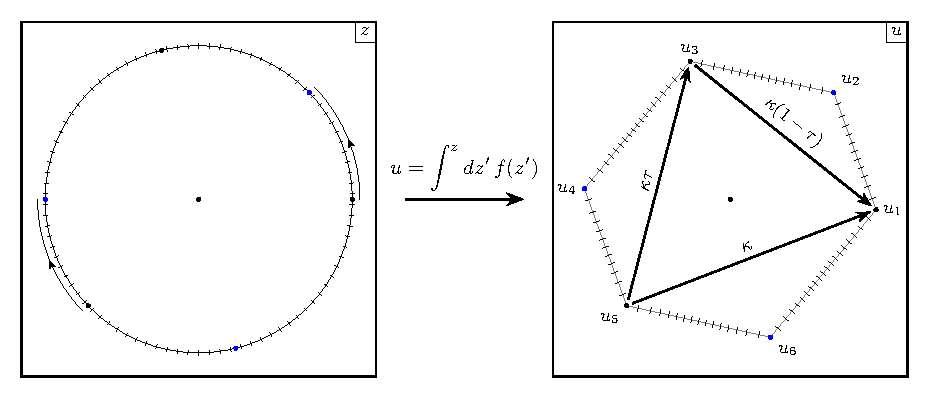
\includegraphics[width=0.8\textwidth]{figures/mapping_diagram.pdf}
  \caption{How $f(z)$ maps the circle to the torus, shown for the specific case of $\ell_i = \{ 11, 15,19\}$. Note that the three black and three blue points correspond to one of the two Strebel vertices, respectively. The arcs in the $z$ plane show how the sides of the cirle are identified with opposite orientation.}
\end{figure}

The flat coordinate on the torus (up to a constant rescaling) can be written as
\ie\label{uflatz}
u = \int^z_{z_0} f(z') dz'
\fe
The metric associated with the ribbon graph is
\ie
{dz d\bar z\over |z|^2} = {du d\bar u \over \left|z \partial_z u \right|^2},
\fe
and so the Weyl factor is given by
\ie
\omega = - \log \left|z f(z)\right|.
\fe
(\ref{slact}) is evaluated as
\ie
S_L &= {1\over 12\pi} \int_{D} d^2z \partial_z \omega \bar\partial_{\bar z} \omega
\\
&= {1\over 12\pi i} \oint_{\partial D} dz\, \omega \partial_z \omega,
\fe
where $D$ is the unit disc with the small neighborhoods of the singular points cut out. The divergent contribution from the component of $\partial D$ near $z=0$ is moduli independent (as $f(0)=1$). Near one of the cubic vertex i.e. zero of Strebel differential, $u=u_i$ ($i=1,2$), we have $\partial_z u = f(z) \approx b_i (u-u_i)^{-{1\over 2}}$, and $\partial_z f(z) = f(z) \partial_u f(z) \approx -{1\over 2} b_i^2 (u-u_i)^{-2}$. It follows that 
\ie
du\, \omega \partial_u \omega\approx - {du\over 4(u-u_i)} \log |f(z)|
\fe
near $u=u_i$. Therefore we have
\ie
S_L = {\log |b_1| + \log |b_2|\over 24} + {\rm universal ~divergence}.
\fe
Here the cutoff is assumed to be $|u-u_i|>\delta$. But should we impose the cutoff on $z$ instead? Near $u=u_i$, we have $z-z_i \approx {2\over 3 b_i} (u-u_i)^{3\over 2}$, and $f(z) \approx b_i ({3b_i\over 2})^{-{1\over 3}} (z-z_i)^{-{1\over 3}} \equiv \nu_i (1-z/z_i)^{-\frac13}$. If we impose the cutoff in $z$, which would seem to be the more compatible with the discretization scheme on the disc, the moduli dependent part of the Weyl anomaly would be given by
\ie
S_L = {\log |b_1| + \log |b_2|\over 36} + {\rm universal ~divergence}.
\fe

\subsection{Special case: $\ell_3=0$}
In the special case when one of the $\ell_i = 0$ (we take $\ell_3=0$ without loss of generality), the corresponding torus has pure imaginary $\tau$, and 
\ie
f(z)dz = \frac{1}{(1-z^2)^{\frac12}(1-z^2 e^{-4i \pi \frac{\ell_1}{L} })^{\frac12}} dz
\fe
exactly. Defining $\theta_1 \equiv 2 \pi \frac{\ell_1}{L}$, the periods of $f$ are given by
\ie
\alpha \text{-cycle: } &e^{i\frac{\theta_1}{2}} K(\cos \frac{\theta_1}{2} )\\
\beta \text{-cycle: } &i e^{i\frac{\theta_1}{2}} K(\sin \frac{\theta_1}{2} )\\
\tau = & i \frac{K(\sin \frac{\theta_1}{2} )}{K(\cos \frac{\theta_1}{2} )}.
\fe
$K(k)$ is the complete elliptic integral of the first kind (\texttt{EllipticK[$k^2$]} in \textbf{Mathematica}). In addition $f(z) \approx \nu_i (z-z_i)^{-\frac12}$, with 
\ie
\nu_i = \frac{1}{\sqrt{\pm4i e^{\mp i \theta_1} \sin \theta_1}}.
\fe
Note that $\nu_1^2 + \nu_2^2 = \frac12$ while $(|\nu_1| + |\nu_2|)^2 = \frac{1}{ \sin(\theta_1) }$.
\section{The $bc$ system}

The identity wave functional of $bc$ system on the unit circle can be written as
\ie
\Psi_1[c(\sigma)] \propto \prod_{n=2}^\infty c_n,
\fe
where $c_n$ is the $n$-th Fourier mode of $c(\sigma)$ (up to a factor of $i$ due to the conformal transformation between cylinder and plane). In the disc coordinate, we can write $c(z) = \sum_{n\in \mathbb{Z}} c_n z^{1-n}$. It follows that $c(z) \Psi_1$ extends holomorphically to the interior of the unit disc, as expected. The analogous ground state wave functionals are
\ie
\Psi_c = c_1 \Psi_1 \propto \prod_{n=1}^\infty c_n,~~~ \Psi_{c\partial c} = c_1 c_0 \Psi_1 \propto  \prod_{n=0}^\infty c_n.
\fe

\fixme{Q: is there a way to make BRST symmetry manifest for the discretized matter+ghost system?}

Now discretizing the unit circle into $L$ sites, we have the approximation
\ie
\Psi_1[c] \propto \prod_{m=2}^{L\over 2} \sum_{k=1}^L c(k) e^{2\pi i {(m-1) k\over L}}.
\fe
Next, we identify pairs of $c(k)$'s according to $k'=s(k)-k$ for $s(k)$ defined in (\ref{shiftRule}). Note that $c(z)$ should transform as a vector field so under $z \to z' = \frac{q}{z}$ for $q$ a phase, ${c(z) \over z} = - {c(z') \over z'}$, i.e. 
\ie
c(k') = - e^{2\pi i \frac{k' - k}{L}} c(k).
\fe
More explicitly
\ie\label{pairthreec}
& c(\tfrac{L}{2} + \ell_1+1 - n) = - e^{\frac{2 \pi i}{L} (\tfrac{L}{2} + \ell_1 + 1 -2n)} c(n),~~~~ 1\leq n \leq \ell_1,
\\
& c(\tfrac{L}{2} + 2 \ell_1 + \ell_2 +1 - n) = -  e^{\frac{2 \pi i}{L} (\tfrac{L}{2} + 2\ell_1 +\ell_2 + 1 -2n)}  c(n),~~~~ \ell_1+1 \leq n \leq \ell_1 + \ell_2,
\\
& c(L+\ell_1 + \ell_2+1 - n) = -  e^{\frac{2 \pi i}{L} (L+ \ell_1 +\ell_2 + 1 -2n)}  c(n),~~~~ \ell_1+\ell_2+1 \leq n \leq \tfrac{L}{2},
\fe
leaving $L\over 2$ independent variables $c(k)$, $k=1, \cdots, {L\over 2}$. We then integrate the constrained $\Psi_1[c]$ over these ${L\over 2}$ independent variables. To obtain a nonzero result requires removing the constant mode of $c$.

Let us consider the constrained $\Psi_c[c]$, which can be put in the form
\ie\label{prodcca}
\prod_{m=1}^{L\over 2} \sum_{k=1}^{L\over 2} B_{mk} c(k).
\fe
The ${L\over 2}\times {L\over 2}$ matrix $B$ is given by 
\ie{}
& B_{mn} =e^{-2\pi i \frac n L} (e^{2\pi i {mn\over L}} - e^{2\pi i {m\over L} (\tfrac{L}{2} + \ell_1+1 - n) }),~~~~ 1\leq n \leq \ell_1,
\\
& B_{mn} = e^{-2\pi i \frac n L} ( e^{2\pi i {mn\over L}} - e^{2\pi i {m\over L} (\tfrac{L}{2} + 2 \ell_1 + \ell_2 +1 - n)}),~~~~ \ell_1+1 \leq n \leq \ell_1 + \ell_2,
\\
& B_{mn} = e^{-2\pi i \frac n L} ( e^{2\pi i {mn\over L}} - e^{2\pi i {m\over L} (L+\ell_1 + \ell_2+1 - n) }),~~~~ \ell_1+\ell_2+1 \leq n \leq \tfrac{L}{2}.
\fe
The result of integrating (\ref{prodcca}) over $c(k)$, $k=1,\cdots,{L\over 2}$, is $\det B$.

The question however is what is the relation between $\det B$ and the torus correlator with appropriate $b,c$ insertions. While there is a $c$ insertion at the center of the disc, there should be a $b$ insertion at the boundary of the disc. Moreover, the $b$ insertion should be localized at the singular points on the boundary of disc where the different segments join. We are after the moduli integration measure
\ie
dt_1 dt_2 \langle {\cal B}_{t_1} {\cal B}_{t_2} c\widetilde c \rangle_{T^2(t_1, t_2)}
\fe
Transforming from the flat coordinate to the disc coordinate via (\ref{uflatz}), we end up with
\ie
dt_1 dt_2 \langle {\cal B}_{t_1} {\cal B}_{t_2} c\widetilde c(0) \rangle_{D^2(t_1, t_2)} |\widehat f(0)|^2,
\fe
where $\widehat f(z)$ is proportional to $f(z)$ of (\ref{fzoneform}), normalized such that the period of $\widehat f(z) dz$ along the $\A$-cycle is 1.

%If we include $bc$ system with 26 free bosons $X^\mu$, so that the Weyl anomalies cancel, we expect the disc frame correlator to give
%\ie
%\langle {\cal B}_{t_1} {\cal B}_{t_2} c\widetilde c(0) \rangle_{D^2(t_1, t_2)}^{X^\mu bc}  \propto {d\tau d\bar\tau\over dt_1 dt_2} |\widehat f(0)|^{-2} \tau_2^{-13} |\eta(\tau)|^{-48}.
%\fe
%The LHS is calculated in the discretized model, up to a moduli-independent normalization factor (that depends on $L$), as
%\ie
%(\det{}' A)^{-13} |\det B|^2.
%\fe

We find that, combining the $bc$ system together with 26 free bosons $X^\mu$, so that Weyl anomalies cancel, that in the disk frame,
\ie
|\det B| ({\det}' A)^{-13} \propto \tau_2^{-13} |\eta(\tau)|^{-48} |\widehat{f} (0)|^{2} \frac{1}{3} \sum_{i=1}^3 \left|\lim_{z\to z_i} (1-\frac{z}{z_i})^{2/3} (\widehat{f}(z))^2\right|^2 .
\fe
In other words, $|\det B|$ calculates the $(\sum_i b(z_i) \wt{b}(\bar{z}_i))c\wt{c}(0)$ correlator on the disk with $c \wt{c}$ inserted at the origin, and $b$ and $\wt{b}$ inserted at the Strebel vertices $z_i$, in the form $\lim_{z\to z_i} (1-\frac{z}{z_i})^{2/3} b(z)$, such that when one considers the transformation to $b(u)$ in the torus coordinate, $ (1-\frac{z}{z_i})^{2/3}$ cancels the divergence of the factors of $f(z)$ that are picked up. Note that in the special case where one of the $\ell_i = 0$, the power must be adjusted to $ (1-\frac{z}{z_i})$.

In the language of \ref{sec:WeylAnomaly}, and denoting the $\alpha$-cycle period of $f(z)$ as $\kappa$, so $\widehat{f}(z) = \frac{1}{\kappa} f(z)$, we can write
\ie
|\det B| ({\det}' A)^{-13} \propto \tau_2^{-13} |\eta(\tau)|^{-48} \frac{1}{|\kappa|^2} \left| \nu \right|^4 ,
\fe
for $\nu$ the average $\nu_i$.
\subsection{Dependence on $c$ position}
Instead of inserting the $c$ ghost at $z=0$ in the disk frame, which gives $\Psi_c[c]$, we can consider $c(z) = \sum_{n \leq 1} c_n z^{1-n}$ inserted at a generic $|z|<1$ and the corresponding $\Psi_{c(z)}[c]$, which will be built from
\ie
\Psi_{c_n}[c] \propto \left(\sum_{k=1}^L c(k) e^{2\pi i \frac{nk}{L}} \right) \prod_{m=2}^{\frac{L}{2}} \left( \sum_{k=1}^L c(k) e^{2\pi i \frac{mk}{L}} \right),
\fe
with the same identification rules \eqref{pairthreec} leaving the usual $\frac{L}{2}$ independent $c(k)$ variables, and resulting in an $\frac{L}{2} \times \frac{L}{2}$ matrix determinant once they are integrated over. We denote this determinant $\det B^{(n)}$, with $\det B^{(1)} = \det B$ of the preceding section.

Clearly, $\det B^{(0)} = 0$ because under \eqref{pairthreec}, the matrix has a zero row. Numerically, we also find that $\det B^{(-n)} = 0$ for even $n$ \fixme{because of the symmetry of the disk under rotation by $\pi$}. In addition, we find that in the case where all three side lengths $\ell_i$ are equal, $\det B^{(n)} = 0$ for all $n \neq 1-6k$ for some $k\in \mathbb{Z}_{\geq 0}$, corresponding to the extra $\mathbb{Z}_6$ rotational symmetry of the disk frame in this special case.

We can define
\ie
g(z) = 1 + \sum_{n=1}^{L/2}{}' \det B^{(-n)} z^{1+n}
\fe
with the $\sum'$ indicating summation over odd $n$. $g(z)$ is proportional to the path integral of $\Psi_{c(z)}[c]$. Considering that the boundary of the unit disc is identified under $z \to z' = q/z$, with $|q|=1$ being three different phases for the three different segments on the boundary, it turns out (numerically tested) that 
\ie
\frac{g(z')}{dz'} = \frac{g(z)}{dz} \quad \Leftrightarrow \quad -\frac{g(z'(z))}{z'} = \frac{g(z)}{z}, \qquad\qquad \text{ for }  |z|=1.
\fe 
Therefore
\ie
g(z) = (f(z))^{-1},
\fe
and $g(z)$ precisely corresponds to the $z$-dependent conformal transformation factor of $c\wt{c}(z,\bar z)$ to the correlator on the disc. The fact that there is seemingly no other $z$-dependence on the position of $c\wt{c}$ implies that there is no extra ghost number 0 $bc$ insertions along the boundary of the disc, besides possibly at the points corresponding to the vertices themselves, in the correlator calculated by the discretized path integral of $\Psi_{c(z)}[c]$.
%implying that the corresponding correlator the path integral is calculating is independent of the insertion position of the $c$-ghost.

%This suggests the following possibility for the correlator when the $\ell_i$ are all equal. In the flat torus coordinate $u$ with $du = f(z) dz$, recall
%\ie
%c^u = \partial_z u ~ c^z = f(z) c^z.
%\fe
%Recall that $f(z(u)) \sim (u-u_i)^{-\frac{1}{2}}$ near the two cubic vertices of the ribbon graph embedded in the flat torus coordinate, and $f(z)$ is identified \textbf{up to change of sign} across the corresponding branch cuts (along the legs of the ribbon graph). It is possible then, that the correlator calculated by the $B$ determinant includes the insertion of 
%\ie
%\exp \left[ i \pi \int_{\gamma_i} dz \, j \right],
%\fe
%where $j = - bc$ is the ghost current and $\gamma_i$ are the segments along the legs of the ribbon graph. This operator must be regularized due to the coincidence of $j$'s from exponentiating the contour, and due to the singularity of $f(z)$ at the vertex points. However, it will pick up the correct compensating phase of $-1$ when a $c$-ghost crosses such a contour. \fixme{what about the ${\cal B}_t$ insertions and any additional ghost-number conserving insertions of $b$ and $c$ on top of that?}

\subsection{Matter and $bc$-ghost on a genus-2 surface}
One can parameterize the genus-2 amplitude via the period matrix $\Omega$ as
\begin{align}
\frac{1}{(\det \im \Omega)^{13}}\frac{1}{|\chi_{10}(\Omega)|^2},
\end{align}
where $\chi_{10}(\Omega)$ is the Igusa-cusp form and $\Omega$ is the period matrix. In the disc frame, the matter +b-c determinant is computed, analogously to the genus 1 case, as 
\begin{align}
\label{eq:numericGenus2}
|\det B| (\det A')^2
\end{align}

Generalizing the genus-1 formula to the case of genus 2, where there are two independent holomorphic one-forms on the boundary, a reasonable guess for the analytic formula of the numerical amplitude in equation \ref{eq:numericGenus2} is
\begin{align}
\frac{1}{(\det \im \Omega)^{13}}\frac{1}{|\chi_{10}(\Omega)|^2}
\end{align}


\section{Free fermion}
The ground-state wavefunction for the free fermion can be written as
\ie
\Psi_1[\psi_r]\propto \prod_{r=\frac{1}{2}}^{\frac{L-1}{2}}\sum_{k=1}^L \psi(k)e^{2\pi i \frac{rk}{L}}
\fe



The fermion is a weight-$\tfrac{1}{2}$ primary, so under sewing together opposite sides of the circle, with $\theta\mapsto-\theta$, the $\psi$ are identified as
\ie{}
&\psi(\tfrac{L}{2}+\ell_1+1-n)=\pm i\psi(n),~~~~1\leq n\leq \ell_1,\\
&\psi(\tfrac{L}{2}+2\ell_1+\ell_2+1-n)=\pm i\psi(n),~~~~\ell_1+1\leq n\leq \ell_1+\ell_2,\\
&\psi(L+\ell_1+\ell_2+1-n)=\pm i\psi(n),~~~~\ell_1+\ell_2+1\leq n\leq \tfrac{L}{2},\\
\fe
where the choice of sign corresponds to the choice of NS/R boundary conditions along the $\alpha,\beta$ cycles.

The constrained $\Psi_1[\psi_r]$ can be put in the form
\ie
\prod_{m=1}^{\frac{L}{2}}\sum_{k=1}^{\frac{L}{2}}D_{mk}\psi(k),
\fe
where the matrix $D$ is given by
\ie{}
D_{mn}&=\exp \left(\tfrac{2\pi i}{L}(m-\tfrac{1}{2})n\right)\pm i\exp\left(\tfrac{2\pi i}{L}(m-\tfrac{1}{2})(\tfrac{L}{2}+\ell_1+1-n)\right),~~~~ 1\leq n \leq \ell_1\\
D_{mn}&=\exp\left(\tfrac{2\pi i}{L}(m-\tfrac{1}{2})n\right)\pm i\exp\left(\tfrac{2\pi i}{L}(m-\tfrac{1}{2})(\tfrac{L}{2}+2\ell_1+\ell_2+1-n)\right),~~~~ \ell_1+1\leq n \leq \ell_1+\ell_2\\
D_{mn}&=\exp\left(\tfrac{2\pi i}{L}(m-\tfrac{1}{2})n\right)\pm i\exp\left(\tfrac{2\pi i}{L}(m-\tfrac{1}{2})(L+\ell_1+\ell_2+1-n)\right),~~~~ \ell_1+\ell_2+1\leq n \leq \frac{L}{2}.\\
\fe

Analagously to the $bc$-ghost correlator, the result of integrating the fermion vacuum wavefunctional over $\psi_r$ is $|\det D|$.

The NS-NS sector amplitude on the flat torus is
\begin{align}
\bigg|\frac{\theta_3(0,\tau)}{\eta(\tau)}\bigg|^2
\end{align}
with similar contributions from the NS/R and R/NS sectors. The Weyl anomaly is $1/2$ the Weyl anomaly of the Empirically, one finds that, proceeding counterclockwise along the bottom segment of the disc, NS/NS corresponds to $-i,-i,+i$, NS/R corresponds to $-i,+i,-i$, and R/NS corresponds to $+i,-i,-i$.

The R/R sector should evaluate to zero without an insertion of the Ramond sector zero mode, which we have not yet inserted.

\section{Higher Genus}

\subsection{Compact boson at higher genus}
For genus 2 surface with 1 puncture, the ribbon graph has 1 face, 6 vertices and 9 edges. There are 4 different topologies of graphs that covers different region of $\mathcal{M}_{2,1}$. Given a ribbon graph, we now describe the algorithm of computing the compact boson partition function on the Riemann surface associated with that ribbon graph. Although we use genus 2 as example, this can be trivially generalized to the case of arbitrary genera.

In order to write down the identification map, Let's label the segments $S_i\ (i=1,...,18)$ from $k=1$ with increasing $k$. The edges can be written as $E_a\ (a=1,...,9)$, where each $E_a$ pairs 2 segments $S_{i_1(a)}, S_{i_2(a)}$ (we always take $i_1(a)<i_2(a)$) and glue them in the opposite orientation. We denote the edge associated with segment $S_i$ by $E_{a(i)}$ and its length $\ell_{a(i)}$. The identification map of compact boson on edge $E_a$ is then:
\ie
X\left(\sum_{j\leq i_1(a)}\ell_{a(j)}+\sum_{k< i_2(a)}\ell_{a(k)}-k+1\right)=X(k)+2\pi R s_a,\quad \sum_{j<i_1(a)}\ell_{a(j)}+1\leq k \leq \sum_{j\leq i_1(a)}\ell_{a(j)}
\fe
One additional complication is that, for higher genus, the independent variables are not simply $X(k)$ with $1\leq k \leq L/2$, since the segments in the same half-circle can be glued together. We take the set of independent variables to be $\mathcal{K}=\cup_{a=1}^9\{k, k\in S_{i_1(a)}\}$, and denote $\mathcal{K}'=\mathcal{K}\backslash \{1\}$.

The condition of no winding around the unit circle can be translated to the following 6 constraints: For each vertex $V_A$, we label the segment that connects to it with the smallest label $S_{i_0(A)}$ (which includes $S_0=S_{18}$), and define
\ie
i_1(A)=i_0(A)+1,\quad  i_2(A)=p(i_1(A))+1,\quad i_3(A)=p(i_2(A))+1
\fe
where $S_{p(i)}$ is the edge paired with $S_i$. The constraints are given by:
\ie
\text{sgn}(i_1(A)) s_{a(i_1(A))}+\text{sgn}(i_2(A)) s_{a(i_2(A))}+\text{sgn}(i_3(A)) s_{a(i_3(A))}=0
\label{constraint}
\fe
where $\text{sgn}(i)$ is defined such that $\text{sgn}(i)=1$ if $i<p(i)$ and $-1$ if $i>p(i)$. In a graph theory way, this can be repacked into a matrix equation
\ie
D_{A,a}s_a=0
\fe
where $s\in \mathbb{Z}^9$ is the vector of 9 shifts and $D\in \mathbb{Z}^{6\times 9}$. The independent shifts then lives in the kernel $\text{ker}_\mathbb{Z}(D)$. If we orient each edge $E_a$ in the counter-clockwise direction of $S_{i_1(a)}$, then the matrix $D$ is then given by the oriented incidence matrix:
\ie
D_{A,a}=\begin{cases}
 1 & \text{if edge } a \text{ into vertex } $A$\\
 -1 & \text{if edge } a \text{ out of vertex } $A$
\end{cases}
\fe
and the dimension of $\text{ker}(D)$ is given by $E-V+1=2g$. Namely, among the 6 constraints, only 5 of them are independent. This reduces the independent number of shifts from 9 to 4, which corresponds to the holonomies around the 4 non-contractible 1-cycles.

A basis of $\text{ker}(D)$ can be built in the following way: One first choose a spanning tree of the oriented graph, which contains $V-1=5$ edges. For each of the 4 edges $e=(A_1(e), A_2(e))$ that's not in the spanning tree, one can find a cycle $C_e$ by starting from $A_1(e)$, going through $e$ to get to $A_2(e)$, then take the unique path in the spanning tree from $A_2(e)$ back to $A_1(e)$. From this cycle $C_e$, one then define a vector
\ie
(b_e)_a=\begin{cases}
 1 & \text{if edge } a \text{ is traversed with same orientation in } C_e\\
 -1 & \text{if edge } a \text{ is traversed with opposite orientation in } C_e\\
 0 & \text{if edge } a \text{ not in } C_e
\end{cases}
\fe
and the 4 $b_e$'s will form a integral basis of $\text{ker}(D)$. If we define the matrix $B\in \mathbb{Z}^{9\times 4}$ by $B_{a,e}=(b_e)_a$, then an arbitrary vector in $\text{ker}(D)$ can be represented by $Bn$, where $n\in \mathbb{Z}^4$ is a lattice vector in the 4-dimensional integral lattice.

The genus-2 compact boson partition function can be discretized as:
\ie
Z^{(2)}(\ell_a;R)=2\pi R \int \prod_{k\in \mathcal{K}} dX(k)\exp\left[-\frac{1}{\pi}\left(\sum_{k,l\in \mathcal{K}'}A_{kl}'X(k)X(l)+2\sum_{k\in\mathcal{K}'}v_k' X(k)+C\right)\right]
\fe
where, similar to \eqref{AvC},
\ie
& A_{kl}=M_{kl}+M_{k'l}+M_{kl'}+M_{k'l'}\\
& A^{'}_{kl}=A_{kl}-A_{1,l}-A_{k,1}-A_{1,1}\\
& v_k=2\pi R\sum_{a=1}^9 s_a \sum_{l\in S_{i_1(a)}}(M_{kl'}+M_{k'l'})\\
v_{k}^{'}=v_{k}-v_1\\
& C=4\pi^2 R^2\sum_{a,b=1}^9 s_a s_b \sum_{k\in S_{i_1(a)}}\sum_{l\in S_{i_1(b)}}M_{k'm'}
\fe
Following the same procedure with the genus-1 case, the partition function can be computed as:
\ie
Z^{(2)}(\ell_a;R)=2\pi R(\det A')^{-1/2}\Theta(4iR^2 T')
\fe
where $T'$ is the following matrix $T_{ab}$ restricted to the 4-dimensional subspace.
\ie
T_{ab}&=\sum_{k\in S_{i_1}(a)}\sum_{l\in S_{i_1}(b)}\left(M_{k'l'}-\sum_{m,n\in \mathcal{K}'}(A')^{-1}_{mn}W_{mk}W_{nl}\right)\\
W_{km}&= M_{km'}+M_{k'm'}-M_{1,m'}-M_{1',m'}
\fe
The restriction from $T$ to $T'$ can be performed by simply taking
\ie
T'=B^T T B
\fe
where the matrix $B^T$ is the one that maps $\mathbb{Z}^9$ to the constrained subspace $\text{ker}(D)$.

At genus $g$, the T-duality transformation of compact boson partition function is given by
\ie
Z^{(g)}(R)=R^{2-2g}Z^{(g)}(R^{-1})
\fe
where the additional factor $R^{2-2g}$ comes from the dilaton shift in the Buscher rules. In terms of the matrix $T'$, this reads
\ie
R^g \Theta(4 i R^2 T')= R^{-g} \Theta(4 i R^{-2} T')
\fe
which has been tested numerically for all 4 topologies of genus 2 and all 818 topologies of genus 3. For genus 4, enumerating and storing all ribbon graph data becomes a problem, but T-duality has been checked for a single topology.

For genus $g$, the compact boson partition function $Z^{(g)}(\Omega, R)$ can be expressed in a lattice sum involving the period matrix $\Omega$:
\ie
Z_\text{comp}^{(g)}(\Omega, R)=2\pi R Z_\text{bos}^{(g)}(\Omega)\sum_{m,n\in \mathbb{Z}^g}\exp\left(-\pi R^2(m+\Omega n)^T(\operatorname{Im}\Omega)^{-1}(m+\bar{\Omega}n)\right)
\fe
where the free boson partition function $Z_\text{bos}(\Omega)$ does not depend on the radius $R$. In term of $T'$,
\ie
\frac{\Theta(4 i R^2_1 T')}{\Theta(4 i R^2_2 T')}=\frac{\sum_{m,n\in \mathbb{Z}^g}\exp\left(-\pi R^2_1(m+\Omega n)^T(\operatorname{Im}\Omega)^{-1}(m+\bar{\Omega}n)\right)}{\sum_{m,n\in \mathbb{Z}^g}\exp\left(-\pi R^2_2(m+\Omega n)^T(\operatorname{Im}\Omega)^{-1}(m+\bar{\Omega}n)\right)}
\fe
and this has been checked for genus 2 using codes in \texttt{compact\_partition.py} and \texttt{ell\_to\_tau.py}.

\subsubsection*{$L$-dependent Renormalization of $Z(\ell_a;R)$}

The lattice constructed provided us a \textit{regularization} scheme, and if we want to have a finite answer when taking the $L\rightarrow \infty$ limit, we need to further \textit{renormalize} the action by adding counterterms. For the theory at self-dual radius $R=1$, we found numerically that the large-$L$ behavior of $Z^{(g)}(\ell_a;R)$ is given by:
\ie
\log Z^{(g)}(L;\Omega;R=1) = c(\Omega) + \gamma L + \alpha(g) \log L
\fe
where $c(\Omega)$ is the moduli-dependent finite part, $\gamma, \alpha(g)$ are both independent of the moduli. $\gamma = \frac{1}{4} \log 2$ is a constant while $\alpha(g)$ is given by the following:
\ie
&\alpha(1)= -1.13889\\
&\alpha(2)= -1.41667\\
&\alpha(3)= -1.69445\\
&\alpha(4)= -1.97222\\
&\alpha(5)= -2.24993
\fe
which suggests that $\alpha(g)$ has a linear dependence in $g$:
\ie
\alpha(g)=\alpha_0+\alpha_1 g,\quad \alpha_0=-0.86112,\quad \alpha_1= - 0.27778
\fe
One can also compute the same large-$L$ dependence for theories with $R\neq 1$ and linear fit the parameters $\alpha(g)$. For theories with different $R$, both the slope and the intercept of $\alpha(g)$ depends on $R$, but $\gamma$ stays the same around $\frac{1}{4} \log 2$.

In order to arrive at a finite partition function in the $L\rightarrow \infty$ limit, we choose the renormalization scheme by adding the following counterterms to the (Euclidean) compact boson action:
\ie
S_\text{counterterm} = \gamma L + (\alpha_0+\alpha_1)\log L- \frac{\alpha_1}{8\pi}\log L\int_\Sigma \mathrm{d}^2\sigma \sqrt{g}\, R(g)
\fe
and the partition function in this renormalization scheme is given by simply $\exp c(\Omega)$.

\section{Analytic construction}

\subsection{Trinion vertex}

The trinion vertex with the three faces of equal circumference $2\pi$ is constructed as 
\ie
\{\Psi_1\otimes \Psi_2\otimes \Psi_3 \}_{[1,1,1]} = \left\langle \prod_{i=1}^3 \left[\Psi_i(0) \right]^{f_i} \right\rangle,
\fe
where $f_i$ are the conformal maps
\ie
f_i =h^{-1}\circ R_i\circ h,
\fe
with
\ie
h(z) \equiv {1+i z\over 1-iz}
\fe
and
\ie
R_1(w) = e^{2\pi i\over 3} w^{2\over 3},~~~~R_2(w) = w^{2\over 3},~~~~R_1(w) = e^{-{2\pi i\over 3}} w^{2\over 3}.
\fe
This construction is analogous to Witten's OSFT cubic vertex. Note however that $\Psi_i$ are not necessarily closed string fields, in that they are not required to obey level matching condition or being annihilated by $b_0^-$.

More generally, we need to consider trinion vertex of face circumferences $2\pi p_i$, $i=1,2,3$, $p_i>0$. Up to permutation, there are two qualitatively distinct cases: (1) $p_1, p_2, p_3$ obey triangular inequality, in which case the ribbon graph is the theta graph, where the three edge lengths $\ell_1, \ell_2, \ell_3$ are related by
\ie
2\pi p_1 = \ell_2 + \ell_3,~~~~ 2\pi p_2 = \ell_3 + \ell_1,~~~~ 2\pi p_3 = \ell_1 + \ell_2,
\fe
and (2) $p_1, p_2, p_3$ do not obey triangular inequality, in which case the ribbon is the dumbbell graph, where the three edge lengths are related by
\ie
2\pi p_1 = \ell_1, ~~~~ 2\pi p_2 = \ell_2,~~~~ 2\pi p_3 = \ell_1 + \ell_2 + 2 \ell_3.
\fe
We will denote the general trinion vertex by
\ie
\{\Psi_1\otimes \Psi_2\otimes \Psi_3 \}_{[p_1,p_2,p_3]} .
\fe
To construct the explicit conformal map, we use the Strebel differential
\ie
\omega = {P(z)\over (z-z_1)^2 (z-z_2)^2 (z-z_3)^2} dz^2,
\fe
where $P(z)$ is a quadratic polynomial in $z$ determined by the conditions 
\ie
{P(z_1)\over z_{12}^2 z_{13}^2} = - {p_1^2},~~~~ {P(z_2)\over z_{21}^2 z_{23}^2}= - {p_2^2},~ ~~{P(z_3)\over z_{31}^2 z_{32}^2} = - {p_3^2}.
\fe
The relevant conformal maps $f_i$ are given by
\ie
f_i^{-1}(z) = \exp\left( {1\over p_i} \int^z \sqrt{\omega} \right),~~~~ z \in D_i,
\fe
where $D_i$ are domains of disc topology that contain $z_i$, such that $f_i$ maps the unit circle to $\partial D_i$. We can then write
\ie
\{\Psi_1\otimes \Psi_2\otimes \Psi_3 \}_{[p_1,p_2,p_3]} = \left\langle \prod_{i=1}^3 \left[\Psi_i(z_i) \right]^{f_i} \right\rangle.
\fe


\subsection{General correlator associated with a ribbon graph}

A general ribbon graph of genus $g$ and $n$ faces can be decomposed into $2g-2+n$ trinion graphs, stitched together with twists. The corresponding correlators can be determined by tracing over internal states with twists. 

For instance, the $(g,n)=(0,4)$ case is given by
\ie
\{\Psi_1\otimes \Psi_2\otimes \Psi_3\otimes \Psi_4 \}^{(0,4)}_{[p_1,p_2,p_3,p_4; x, y]} = \sum_I \{\Psi_1\otimes \Psi_2\otimes e^{2\pi i L_0^- y} \phi_I \}_{[p_1,p_2,x]}  \{\phi_I^\vee \otimes \Psi_3\otimes \Psi_4  \}_{[x,p_3,p_4]},
\fe
where $\phi_I$ and $\phi_I^\vee$ are dual bases (with respect to BPZ inner product) of the worldsheet CFT state space. The underlying ribbon graph has 4 vertices, 6 edges, 4 faces. 

For $(p_1, p_2, x)$ and $(p_3, p_4, x)$ obeying triangular inequalities, the 6 edge lengths $\ell_i$ are related by
\ie{}
& 2\pi p_1 = \ell_1 + \ell_2 + \ell_3,
\\
& 2\pi p_2 = \ell_1 + \ell_4 + \ell_5,
\\
& 2\pi p_3 = \ell_3 + \ell_4 + \ell_6,
\\
& 2\pi p_4 = \ell_2 + \ell_5 + \ell_6,
\\
& 2\pi x = \ell_2 + \ell_3 + \ell_4 + \ell_5,
\\
& 2\pi y = \ell_2.
\fe
In other cases, the underlying ribbon graph may also involve a dumbbell subgraph.

As another example, for $(g, n) = (1,1)$, we have
\ie
\{\Psi\}^{(1,1)}_{[p; x,y]} = \sum_I  \{\Psi\otimes e^{2\pi i L_0^- y}\phi_I\otimes \phi_I^\vee \}_{[p,x,x]} .
\fe
Here $p>2x$. The underlying ribbon graph has 2 vertices, 3 edges, 1 face. It is formed out of self-plumbing of a dumbell graph, whose edge lengths $\wt\ell_1, \wt\ell_2, \wt\ell_3$ are related by
\ie
2\pi p = 2 \wt\ell_1 + \wt\ell_2 + \wt\ell_3 ,
~~~~ 2\pi x = \wt\ell_2 = \wt\ell_3.
\fe
The $(g,n)=(1,1)$ ribbon graph has three edges of length $\ell_1, \ell_2, \ell_3$, related by
\ie
\ell_1 = \wt\ell_1 ,~~~~ \ell_2 = y,~~~~  \ell_3 = \wt\ell_2 - y.
\fe
Note that $\ell_1 + \ell_2 + \ell_3 = \wt\ell_1 + \wt \ell_2 = \pi p$.




\end{document}






































